\documentclass[12pt]{amsproc}

% a la fullpage
\usepackage{geometry}
\geometry{a4paper}
\geometry{twoside=false}

% Activate to begin paragraphs with an empty line rather than an indent
\usepackage[parfill]{parskip}
\setlength{\marginparwidth}{2cm}

\theoremstyle{plain}
\newtheorem{theorem}{Theorem}[section]
\newtheorem{proposition}[theorem]{Proposition}
\newtheorem{lemma}[theorem]{Lemma}
\newtheorem{corollary}[theorem]{Corollary}

\theoremstyle{definition}
\newtheorem{definition}[theorem]{Definition}
\newtheorem{example}[theorem]{Example}
\newtheorem{exlemma}[theorem]{Example/Lemma}

\usepackage{graphicx}
\usepackage{float}
\usepackage{amssymb}
\usepackage{color}
\usepackage{listings}

%\newcommand{\id}{\text{id}}
\newcommand{\N}{\mathbb{N}}
\newcommand{\Z}{\mathbb{Z}}
\newcommand{\R}{\mathbb{R}}
\newcommand{\cat}[1]{\mathbf{#1}}
\newcommand{\Ab}{\cat{Ab}}
\newcommand{\sAb}{\cat{sAb}}
\newcommand{\Set}{\cat{Set}}
\newcommand{\Ch}[1]{\mathbf{Ch}(#1)}
\newcommand{\Hom}[3]{\mathbf{Hom}_{#1}(#2, #3)}
\newcommand{\id}{\mathbf{id}}

\newcommand{\iso}{\cong}
\newcommand{\tot}[1]{\xrightarrow{\,\,{#1}\,\,}}
\newcommand{\eps}{\varepsilon}
\newcommand{\I}{\,\mid\,}
\newcommand{\then}{\Rightarrow}
\newcommand{\inject}{\hookrightarrow}
\newcommand{\del}{\partial}
\newcommand{\nsubgrp}{\trianglelefteq}

% relative to the one who includes us :(
\graphicspath{ {../images/} }

\newcommand{\todo}[1]{
	\addcontentsline{tdo}{todo}{\protect{#1}}
	$\ast$ \marginpar{\tiny $\ast$ #1}
}
\makeatletter
	\newcommand \listoftodos{\section*{Todo list} \@starttoc{tdo}}
	\newcommand\l@todo[2]{
		\par\noindent \textit{#2}, \parbox{10cm}{#1}\par
	}
\makeatother

\graphicspath{ {../thesis/images/}, {../presentation/images/} }

\title{Dold-Kan Correspondence}
\author{Joshua Moerman}

\begin{document}
\maketitle

\section*{Introduction}
In this thesis we will look at a correspondence which was discovered by A. Dold and D. Kan independently, hence it is called the \emph{Dold-Kan correspondence}. Abstractly it is the following equivalence of categories:
$$ \Ch{\Ab} \simeq \sAb $$
It is interesting because objects on the left hand side are considered to be algebraic of nature, whereas objects on the right are more topological. In particular this correspondence also gives a isomorphism between homology groups (on the left hand side) and homotopy groups (on the right hand side). A bit more precise:
$$ \pi_n(A) \iso H_n(N(A)) \text{ for all } n \in \N $$
where $N: \sAb \to \Ch{\Ab}$ is one half of the equivalence.

In the first section some definitions from category theory are given, because we will need them later on. Then in the second section we will discuss the first category involved in the correspondence, $\Ch{\Ab}$, the category of chain complexes. The third section then continues with the second category involved, $\sAb$, especially for this section we will need category theory. Then we will look at the coorespondence itself.

\newpage
\section{Category Theory}
\label{sec:Category Theory}
Before we will introduce the two categories $\Ch{\Ab}$ and $\sAb$, we will first look at some basic category theory. If one is already familier with these concepts, he or she can skip this section. We will introduce the notions of categories, functors, isomorphims, natural transformations, equivalences (between categories) and adjunctions.

\subsection{Categories}
\begin{definition}
	A \emph{category} $\cat{C}$ consists of a collection \emph{objects}, and for each two objects $A$ and $B$ in $\cat{C}$ there is a (possibly empty) \emph{set of maps} (or arrows) from $A$ to $B$, notated as $\Hom{\cat{C}}{A}{B}$, such that:
	\begin{itemize}
		\item \emph{(Identity)}
			$\id_A \in \Hom{\cat{C}}{A}{A}$ for all $A$ in $\cat{C}$,
		\item \emph{(Composition)}
			for any $f \in \Hom{\cat{C}}{A}{B}$ and $g \in \Hom{\cat{C}}{B}{C}$ we have $g \circ f \in \Hom{\cat{C}}{A}{C}$,
		\item \emph{(Associativity)}
			$f \circ (g \circ h) = (f \circ g) \circ h$, and
		\item \emph{(Identity law)}
			$\id_B \circ f = f = f \circ \id_A$ for all $f \in \Hom{\cat{C}}{A}{B}$.
	\end{itemize}
\end{definition}

Note that the collection of objects may be a proper class instead of a set, however we will notate $A \in \cat{C}$ if $A$ is an object of $\cat{C}$. And instead of writing $f \in \Hom{\cat{C}}{A}{B}$, we write $f: A \to B$.

As the notation suggests maps can be thought of as functions, which is also the case in many examples.

\begin{lemma}
	The category $\Set$ has a objects sets, and as maps ordinary functions. Of course we then have the identity function $\id_X(x) = x$ and composition as usual.
\end{lemma}
\begin{lemma}
	The category $\Ab$ has a objects abelian groups, and the maps between two objects are exactly the grouphomomorphisms. We know that the identity function is indeed a grouphomomorphism, and composing two grouphomomorpisms, gives indeed a new grouphomomorphism.
\end{lemma}

In fact almost any mathematical structure can be described as a category, we have: $\cat{Ring}$ for rings, $\cat{Vect}$ for $\R$-vectorspaces, $\cat{Set_{fin}}$ for finite sets, $\cat{Poset}$ for posets, etc. Of course we would also like to express relations between categories, for example every abelian group is also a set. This idea can be formulated by the notion of a functor.

\begin{definition}
	A \emph{functor} $F$ between a category $\cat{C}$ and $\cat{D}$ consists of a function $F_0$ from the objects of $\cat{C}$ to the objects of $\cat{D}$ and a function $F_1$ from maps in $\cat{C}$ to maps in $\cat{D}$, such that:
	\begin{itemize}
		\item for $f: A \to B$, we have $F_1(f): F_0(A) \to F_0(B)$,
		\item $F_1(\id_A) = \id_{F_0(A)}$ and
		\item $F_1(f \circ g) = F_1(f) \circ F_1(g)$.
	\end{itemize}
	We normally do not write the index of $F_0$ or $F_1$, instead we wrtie $F$ for both functions.
\end{definition}

\begin{lemma}
	There is a category $\cat{Cat}$ with categories as objects, and functors as maps.
\end{lemma}
\begin{proof}
	First we define the identity functor. Let $\cat{C}$ be a category, define $\id_\cat{C}(A) = A$ for any object $A \in \cat{C}$ and $\id_\cat{C}(f) = f$ for any map $f: A \to B$ in $\cat{C}$. Cleary we have $\id_\cat{C}(f) : \id_\cat{C}(A) \to \id_\cat{C}(B)$. Also $\id_\cat{C}(\id_A) = \id_A = \id_{\id_\cat{C}(A)}$ and $\id_\cat{C}(f \circ g) = f \circ g$. So indeed $\id_\cat{C}$ is a functor.

	Given a functors $F: \cat{C} \to \cat{D}$ and $G: \cat{D} \to \cat{E}$, we can define the composition $G \circ F$ on objects as $G \circ F(A) = G(F(A))$ and on maps as $G \circ F(f) = G(F(f))$. This again is a functor $G \circ F$, we will not spell out the details.

	The remaining requirements are the associativity and identity law. We also leave these to the reader.
\end{proof}

\subsection{Isomorphisms}
Given a category $\cat{C}$ and two objects $A, B \in \cat{C}$ we would like to know when those objects are regarded as the same, according to the category. This will be the case when there is an isomorphism between the two.

\begin{definition}
	A map $f: A \to B$ in a category $\cat{C}$ is an isomorphism if there is a map $g: B \to A$ such that:
	$$ f \circ g = \id_B \text{ and } g \circ f = id_A.$$
\end{definition}

Isomorphisms in $\Ab$ are exactly the isomorphisms which we know, ie. the grouphomomorphisms which are both injective and surjective.
For example the cyclic group $\Z_4$ and the klein four-group $V_4$ are not isomorphic in $\Ab$, but if we regard only the sets $\Z_4$ and $V_4$, then they are (because there is a bijection). So it is good to note that whether two objects are isomorphic  really depends on the category we are working in.

\todo{CT: Equivalence / natro}
\todo{CT: Adjunction}


\newpage
\section{Chain Complexes}
\label{sec:Chain Complexes}
\begin{definition}
	A \emph{(non-negative) chain complex} $C$ is a collection of abelian groups $C_n$ together with group homomorphisms $\del_n: C_n \to C_{n-1}$, which we call \emph{boundary homomorphisms}, such that $\del_n \circ \del_{n+1} = 0$ for all $n \in \Np$.
\end{definition}

Thus graphically a chain complex $C$ can be depicted by the following diagram:
\begin{center}
\begin{tikzpicture}
	\matrix (m) [matrix of math nodes]{
		\cdots & C_4 & C_3 & C_2  & C_1 & C_0 \\
	};
	\foreach \d/\i/\j in {5/1/2,4/2/3,3/3/4,2/4/5,1/5/6} \path[->] (m-1-\i) edge node[auto] {$ \del_\d $} (m-1-\j);
\end{tikzpicture}
\end{center}

There are many variants to this notion. For example, there are also unbounded chain complexes with an abelian group for each $n \in \Z$ instead of $\N$. In this thesis we will only need chain complexes in the sense of the definition above. Hence we will simply call them chain complexes, instead of non-negative chain complexes. Other variants can be given by taking a collection of $R$-modules instead of abelian groups. Of course not any kind of mathematical object will suffice, because we need to be able to express $\del_n \circ \del_{n+1} = 0$, so we need some kind of \emph{zero object}. We will not need this kind of generality and stick to abelian groups.

In order to organize these chain complexes in a category, we should define what the maps are. The diagram above already gives an idea for this.
\begin{definition}
	Let $C$ and $D$ be chain complexes, with boundary maps $\del^C_n$ and $\del^D_n$ respectively. A \emph{chain map} $f: C \to D$ consists of a family of maps $f_n: C_n \to D_n$, such that they commute with the boundary operators: $f_n \circ \del^C_{n+1} = \del^D_{n+1} \circ f_{n+1}$ for all $n \in \N$, i.e. the following diagram commutes:
	\begin{center}
	\begin{tikzpicture}
		\matrix (m) [matrix of math nodes]{
			\cdots & C_4 & C_3 & C_2  & C_1 & C_0 \\
			\cdots & D_4 & D_3 & D_2  & D_1 & D_0 \\
		};
		\foreach \d/\i/\j in {5/1/2,4/2/3,3/3/4,2/4/5,1/5/6} \path[->] (m-1-\i) edge node[auto] {$ \del^C_\d $} (m-1-\j);
		\foreach \d/\i/\j in {5/1/2,4/2/3,3/3/4,2/4/5,1/5/6} \path[->] (m-2-\i) edge node[auto] {$ \del^D_\d $} (m-2-\j);
		\foreach \d/\i in {4/2,3/3,2/4,1/5,0/6} \path[->] (m-1-\i) edge node[auto] {$ f_\d $} (m-2-\i);
	\end{tikzpicture}
	\end{center}
\end{definition}

Note that if we have two such chain maps $f:C \to D$ and $g:D \to E$, then the levelwise composition will give us a chain map $g \circ f: C \to D$. Also taking the identity function in each degree, gives us a chain map $\id : C \to C$. In fact, this will form a category, we will leave the details (the identity law and associativity) to the reader.

\begin{definition}
	$\Ch{\Ab}$ is the category of chain complexes with chain maps.
\end{definition}

Note that we will often drop the indices of the boundary morphisms, since it is often clear in which degree we are working. The boundary operators give rise to certain subgroups, because all groups are abelian, subgroups are normal subgroups.

\begin{definition}
	Given a chain complex $C$ we define the following subgroups:
	\begin{itemize}
		\item $Z_n(C) = \ker(\del_n: C_n \to C_{n-1}) \nsubgrp C_n$, and
		\item $Z_0(C) = C_0$, and
		\item $B_n(C) = \im(\del_{n+1}: C_{n+1} \to C_n) \nsubgrp C_n$.
	\end{itemize}
\end{definition}
\begin{lemma}
	Given a chain complex $C$ we have for all $n \in \N$:
	$$ B_n(C) \nsubgrp Z_n(C).$$
\end{lemma}
\begin{proof}
	It follows from $\del_n \circ \del_{n+1} = 0$ that $\im(\del: C_{n+1} \to C_n)$ is a subset of $\ker(\del: C_n \to C_{n-1})$. Those are exactly the abelian groups $B_n(C)$ and $Z_n(C)$, so $ B_n(C) \nsubgrp Z_n(C) $.
\end{proof}
\begin{definition}
	Given a chain complex $C$ we define the \emph{$n$-th homology group} $H_n(C)$ for each $n \in \N$ as:
	$$ H_n(C) = Z_n(C) / B_n(C).$$
\end{definition}

\todo{CC: $H_n$ as a functor} 

\subsection{The singular chain complex}
In order to see why we are interested in the construction of homology groups, we will look at an example from algebraic topology. We will see that homology gives a nice invariant for spaces. So we will form a chain complex from a topological space $X$. In order to do so, we first need some more notions.
\begin{definition}
	The topological space $\Delta^n$ is called the \emph{topological $n$-simplex} and is defined as:
	$$ \Delta^n = \{(x_0, x_1, \ldots, x_n) \in \R^{n+1} \I x_i \geq 0 \text{ and } x_0 + \ldots + x_n = 1 \}.$$
	The topology on $\Delta^n$ is the subspace topology.
\end{definition}

In particular $\Delta^0$ is simply a point, $\Delta^1$ a line and $\Delta^2$ a triangle. There are nice inclusions $\Delta^n \mono \Delta^{n+1}$ which we need later on. For any $n \in \N$ we define:
\begin{definition}
	For $i \in \{0, \ldots, n+1\}$ the $i$-th face map $\delta^i : \Delta^n \mono \Delta^{n+1}$ is defined as:
	$$ \delta^i (x_0, \ldots, x_n) = (x_0, \ldots, x_{i}, 0, x_{i+1}, \ldots, x_n) \text{ for all } x \in \Delta^n.$$
\end{definition}

For any space $X$, we will be interested in continuous maps $\sigma : \Delta^n \to X$, such a map is called a $n$-simplex. Note that if we have any continuous map $\sigma : \Delta^{n+1} \to X$ we can precompose with a face map to get $\sigma \circ \delta^i : \Delta^n \to X$, as shown in figure~\ref{fig:diagram_d}. This will be used for defining the boundary operator. We can make pictures of this, and when concerning continuous maps $\sigma : \Delta^{n+1} \to X$ we will draw the images in the space $X$, instead of functions.

\begin{figure}
	\begin{tikzpicture}
		\matrix (m) [matrix of math nodes]{
			\Delta^{n+1} & X \\
			\Delta^n & \\
		};
		\path[->]
		(m-1-1) edge node[auto] {$ \sigma $} (m-1-2)
		(m-2-1) edge node[auto] {$ \delta^i $} (m-1-1)
		(m-2-1) edge node[auto] {$ $} (m-1-2);
	\end{tikzpicture}
	\caption{The $(n+1)$-simplex $\sigma$ can be made into a $n$-simplex $\sigma \circ \delta^i$}
	\label{fig:diagram_d}
\end{figure}

\todo{Ch: Make some pictures here}

We now have enough tools to define the singular chain complex of a space $X$.

\begin{definition}
	For a topological space $X$ we define the \emph{$n$-th singular chain group} $C_n(X)$ as follows.
	$$ C_n(X) = \Z[\Hom{\cat{Top}}{\Delta^n}{X}] $$
	The boundary operator $\del : C_{n+1}(X) \to C_n(X)$ is defined on generators as:
	$$ \del(\sigma) = \sigma \circ \delta^0 - \sigma \circ \delta^1 + \ldots + (-1)^{n+1} \sigma \circ \delta^{n+1}.$$
\end{definition}

This might seem a bit complicated, but we can pictures this in an intuitive way, as in figure~\ref{fig:singular_chaincomplex3}. And we see that the boundary operators really give the boundary of an $n$-simplex. To see that this indeed is a chain complex we have to proof that the composition of two such operators is the zero map.
\begin{figure}[h!]
	\includegraphics{singular_chaincomplex3}
	\caption{The boundary of a 2-simplex}
	\label{fig:singular_chaincomplex3}
\end{figure}
\todo{CC: update picture}

\todo{Ch: Proposition: $C(X) \in \Ch{\cat{Ab}}$}
\todo{Ch: Example homology of some space}
\todo{Ch: Show that $\Ch{\Ab}$ is an ab. cat. At least show functoriality $\Hom{\Ch{\Ab}}{-}{-}$}


\newpage
\section{Simplicial Abelian Groups}
\label{sec:Simplicial Abelian Groups}

Before defining \emph{simplicial abelian groups}, we will first discuss the more general notion of \emph{simplicial sets}. There are generally two definitions of simplicial sets, an abstract one and a very explicit one. We will start with the abstract one, luckily it can still be visualised in pictures, then we will derive the explicit definition. The reader who is interested in how these notions developed, should consider reading the introduction by Friedman \cite{friedman}, which also gives nice illustrations.

\subsection{Abstract definition}
\begin{definition}
	We define a category $\DELTA$, where the objects are the finite ordinals $[n] = \{0, \dots, n\}$ for $n \in \N$ and maps are monotone increasing functions: $\Hom{\DELTA}{[n]}{[p]} = \{ f : [n] \to [p] \I f(i) \leq f(j) \text{ for all } i < j \}$.
\end{definition}

There are two special kinds of maps in $\DELTA$, the so called \emph{face} and \emph{degeneracy} maps. The $i$-th face maps $\delta_i$ is the unique injective monotone increasing function which \emph{omits} $i$. More precisely it is defined for all $n \in \Np$ as (note that we do not explicitly denote $n$ in this notation):
$$ \delta_i: [n-1] \to [n], k \mapsto \begin{cases} k & \text{if } k < i;\\ k+1 & \text{if } k \geq i. \end{cases} \hspace{0.5cm} 0 \leq i \leq n. $$

The $i$-th degeneracy map $\sigma_i$ is the unique surjective monotone increasing function which hits $i$ twice. More precisely it is defined for all $n \in \N$ as:
$$ \sigma_i: [n+1] \to [n], k \mapsto \begin{cases} k & \text{if } k \leq i;\\ k-1 & \text{if } k > i. \end{cases} \hspace{0.5cm} 0 \leq i \leq n. $$

The nice things about these maps is that every map in $\DELTA$ can be decomposed to a composition of these maps. So in a sense, these are all the maps we need to consider.

\begin{lemma}
	\label{le:epimono}
	Let $\eta : [m] \to [n]$ be a map in $\DELTA$. Then $\eta$ can be uniquely decomposed as:
	$$ \eta = \delta_{i_a} \cdots \delta_{i_1} \sigma_{j_b} \cdots \sigma_{j_1}, $$
	such that $0 \leq j_b < \cdots < j_1 < m$ and $0 \leq i_1 < \cdots < i_a \leq n$.
\end{lemma}
\begin{proof}
	We start with the existence. Consider the set $S = \{ k \in [m-1] \I \eta(k) = \eta(k+1) \}$. These are precisely the elements which are hit twice, now let $S = \{ j_1, \ldots, j_{|S|} \}$ with $0 \leq j_{|S|} < \cdots < j_1 < m$. This gives rise to a surjection $\sigma = \sigma_{j_b} \cdots \sigma_{j_1}: [m] \epi [m-|S|]$.

	Similarly consider $T = \{ k \in [m - |S|] \I k \not \in \eta[m] \}$. These are precisely the elements which are omitted, now let $T = \{ i_1, \ldots, i_{|T|} \}$ with $0 \leq i_1 < \cdots < i_{|T|} \leq n$. This gives an injection $\delta = \delta_{i_a} \cdots \delta_{i_1} : [m - |S|] \mono [n]$. Now we see that $\eta = \delta\sigma$.

	Now for uniqueness, \todo{sAb: uniqueuness epi-mono}
\end{proof}

We can now picture the category $\DELTA$ as in figure~\ref{fig:delta_cat}. Note that the face and degeneracy maps are not unrelated. We will make the exact relations precise later.

\begin{figure}[h!]
	\includegraphics{delta_cat}
	\caption{The category $\DELTA$ with the face and degeneracy maps.}
	\label{fig:delta_cat}
\end{figure}

Although this is a very abstract definition, a more geometric intuition can be given. In $\DELTA$ we can regard $[n]$ as an abstract version of the $n$-simplex $\Delta^n$. The face maps $\delta_i$ are then exactly maps which point out how we can embed $[n]$ in $[n+1]$. This is shown in figure~\ref{fig:delta_cat_geom}. This picutre shows the images of the face maps, for example the image of $\delta_3$ from $[2]$ to $[3]$ is the set $\{0,1,2\}$, which is the bottom face of the tetrahedron. The degeneracy maps are harder to visualize, one can think of them as ``collapsing'' maps, where two points are identified with each other. For example, this collapses a triangle into a line.

\begin{figure}
	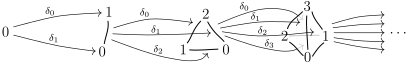
\includegraphics{delta_cat_geom}
	\caption{The category $\DELTA$ with the face maps shown in a geometric way.}
	\label{fig:delta_cat_geom}
\end{figure}

This category $\DELTA$ will act as a protoype for these kind of geometric structures in other categories. This leads to the following definition.

\begin{definition}
	A \emph{simplicial set} $X$ is a functor:
	$$X: \DELTA^{op} \to \Set.$$
	(Or equivalently a contravariant functor $X: \DELTA \to \Set.$)
\end{definition}

So the category of all simplicial sets, $\sSet$, is the functor category $\Set^{\DELTA^{op}}$, where morphisms are natural transformations. Because the face and degeneracy maps give all the maps in $\DELTA$ it is sufficient to define images of $\delta_i$ and $\sigma_i$ in order to define a functor $X: \DELTA^{op} \to \Set$, keep in mind that these should satisfy some relations which we will discuss next. Hence we can picture a simplicial set as done in figure~\ref{fig:simplicial_set}. Comparing this to figure~\ref{fig:delta_cat} we see that the arrows are reversed, because $X$ is a contravariant functor.

\begin{figure}
	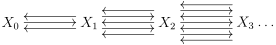
\includegraphics{simplicial_set}
	\caption{A simplicial set.}
	\label{fig:simplicial_set}
\end{figure}


\subsection{Explicit definition}
Of course the maps $\delta_i$ and $\sigma_i$ in $\DELTA$ satisfy certain relations, these are the so called \emph{cosimplicial identities}.

\begin{lemma}
	The face and degeneracy maps in $\DELTA$ satisfy the cosimplicial identities, i.e.:
	\begin{align}
		\delta_j\delta_i &= \delta_i\delta_{j-1}  \hspace{0.5cm} \text{ if } i < j,\\
		\sigma_j\delta_i &= \delta_i\sigma_{j-1}  \hspace{0.5cm} \text{ if } i < j,\\
		\sigma_j\delta_j &= \sigma_j\delta_{j+1} = \id,\\
		\sigma_j\delta_i &= \delta_{i-1}\sigma_j  \hspace{0.5cm} \text{ if } i > j+1,\\
		\sigma_j\sigma_i &= \sigma_i\sigma_{j+1}  \hspace{0.5cm} \text{ if } i \leq j.
	\end{align}
\end{lemma}
\begin{proof}
	By writing out the definitions given above. \todo{sAb: this is a bit rude, maybe write out some of it...}
\end{proof}

Because a simplicial set $X$ is a contravariant functor, these equations (which only consist of compositions and identities) also hold in its image. For example the first equation would look like: $ X(\delta_i)X(\delta_j) = X(\delta_{j-1})X(\delta_i) $ for $ i < j$. This can be used for an explicit definition of simplicial sets. In this definition a simplicial set $X$ consists of a collection sets $X_n$ together with the face and degeneracy maps. More precisely:

\begin{definition}
	\emph{(Explicitly)} An simplicial set $X$ consists of a collection sets $X_n$ together with functions $d_i : X_n \to X_{n-1}$ and $s_i : X_n \to X_{n+1}$ for $0 \leq i \leq n$ and $n \in \N$, such that the simplicial identities hold:
	\begin{align}
		d_i d_j &= d_{j-1} d_i  \hspace{0.5cm} \text{ if } i < j,\\
		d_i s_j &= s_{j-1} d_i  \hspace{0.5cm} \text{ if } i < j,\\
		d_j s_j &= d_{j+1} s_j = \id,\\
		d_i s_j &= s_j d_{i-1}  \hspace{0.5cm} \text{ if } i > j+1,\\
		s_i s_j &= s_{j+1} s_i  \hspace{0.5cm} \text{ if } i \leq j.
	\end{align}
\end{definition}

It is already indicated that a functor from $\DELTA^{op}$ to $\Set$ is determined when the images for the face and degeneracy maps in $\DELTA$ are provided. So this gives a way of restoring the first definition from this one. Conversely, we can apply functorialty to obtain the second definition from the first. So these definitions are the same. From now on we will denote $X([n])$ by $X_n$, $X(\sigma_i)$ by $s_i$ and $X(\delta_i)$ by $d_i$, whenever we have a simplicial set $X$. For any other map $\beta : [n] \to [p]$ we will denote the induced map by $\beta^\ast : X_p \to X_n$.

When using a simplicial set to construct another object, it is often handy to use this second definition, as it gives you a very concrete objects to work with. On the other hand, constructing this might be hard (as you would need to provide a lot of details), in this case we will often use the more abstract definition.

Note that because of the third equation, the degeracy maps $s_i$ are injective. This means that in the set $X_{n+1}$ there are always ``copies'' of elements of $X_n$. In a way these elements are not interesting, hence we call them degenerate.
\begin{definition}
	An element $x \in X_{n+1}$ is \emph{degenerate} if it lies in the image of $s_i : X_n \to X_{n+1}$ for some $i$. An element is called \emph{non-degenerate} if this is not the case.
\end{definition}
\begin{lemma}
	We can write any $x \in X_n$ uniquely as $x = \beta^\ast y$ for some surjective map $\beta : [n] \epi [m]$ and $y \in X_m$ non-degenerate.
\end{lemma}
\begin{proof}
	We will proof the existence with inducion over $n$. For $n=0$ the statement is trivial, since all elements in $X_0$ are non-degenerate. Assume the statement is proven for $n$. Let $x \in X_{n+1}$. Clearly if $x$ itself is non-degenerate, we can write $x = \id^\ast x$. Otherwise it is of the form $x = s_i x'$ for some $x' \in X_n$ and $i$. The induction hypothesis tells us that we can write $x' = \beta^\ast y$ for some surjection $\beta: [n] \epi [m]$ and $y \in X_m$ non-degenerate. So $x = s_i \beta^\ast y = (\beta \sigma_i)^\ast y$.

	For uniqueness, assume $x = \beta^\ast y = \gamma^\ast z$ with $\beta : [n] \epi [m]$, $\gamma: [n] \epi [m']$ and $y \in X_m, z \in X_{m'}$ non-degenerate. Because $\beta$ is surjective there is an $\alpha:[m]\to[n]$ such that $\beta\alpha = \id$ and hence $y = \alpha^\ast \gamma^\ast z = (\gamma\alpha)^\ast z$. By lemma~\ref{le:epimono} we can write $\gamma\alpha = \delta_{i_a} \cdots \delta_{i_1} \sigma_{j_b} \cdots \sigma_{j_1}$, using that $y$ is non-degenerate we know that $\gamma\alpha$ is injective. So we have $\gamma\alpha: [m] \mono [m']$. Because of symmetry (of $y$ and $z$) we also have some map $[m'] \mono[m]$, so $m = m'$. So $\gamma\alpha$ is also surjective, hence the identity function, thus $y = z$.
	\todo{sAb: $\gamma = \beta$}
\end{proof}

\subsection{The standard $n$-simplex}
Recall that for any category $\cat{C}$ we have the $\mathbf{Hom}$-functor: $\Hom{\cat{C}}{-}{-} : \cat{C}^{op} \times \cat{C} \to \Set$. We can fix an object $C \in \cat{C}$ and get a functor $\Hom{\cat{C}}{-}{C} : \cat{C}^{op} \to \Set$. In our case we can get the following simplicial sets in this way:

\begin{definition}
	The standard $n$-simplex is given by:
	$$\Delta[n] = \Hom{\DELTA}{-}{[n]} : \DELTA^{op} \to \Set.$$
\end{definition}

Note that this is also the definition of the Yoneda embedding $\Delta[n] = y[n]$. In a moment we will see why the Yoneda lemma is useful to us. But we will explicitly describe two of such standaard $n$-simplices.

\begin{example}
	We will compute how $\Delta[0]$ look like. Note that $[0]$ is an one-element set, so for any set $X$, there is only one function $\ast : X \to [0]$. Hence $\Delta[0]_n = \{\ast\}$ for all $n$. The face and degeneracy maps are now functions from $\{\ast\}$ to $\{\ast\}$. Again there is only one, namely $\id : \{\ast\} \to \{\ast\}$. This gives:
	$$ \Delta[0] = \{\ast\} \to \{\ast\} \to \{\ast\} \to \cdots. $$
	Note that the only non-degenerate simplex is the unqiue $0$-simplex.
\end{example}

\begin{example}
	$\Delta[1]$ is a bit more interesting, but still not too hard. We will compute the first three abelian groups $\Delta[1]_0$, $\Delta[1]_1$ and $\Delta[1]_2$. We can use the fact that any monotone increasing map $f: [n] \to [m]$ is a composition of first applying degeneracy maps, and then face maps, ie.: $f: [n] \tot{\sigma_{i_0} \cdots \sigma_{i_M}} [k] \tot{\delta_{j_0} \cdots \delta_{j_N}} [m]$, where $k \leq m, n$.

	For $\Delta[1]_0$ we have to consider maps from $[0]$ to $[1]$, we cannot first apply degeneracy maps (there is no object $[-1]$). So this leaves us with the face maps: $\Delta[1]_0 = \{\delta_0, \delta_1\}$. For $\Delta[1]_1$ we of course have the identity function and two functions $\delta_0\sigma_0, \delta_1\sigma_0$. Now $\Delta[1]_2$ are the maps from $[2]$ to $[1]$.

	We will compute the two face maps $d_0$ and $d_1$ from $\Delta[1]_1$ to $\Delta[1]_0$. Recall that the $\mathbf{Hom}$-functor in the first argument (the contravariant argument) works with precomposition. So this gives:
	\begin{align*}
		d_0(id) &= \id \delta_0 = \delta_0 \\
		d_0(\delta_0\sigma_0) &= \delta_0 \sigma_0 \delta_0 = \delta_0 \\
		d_0(\delta_1\sigma_0) &= \delta_0 \sigma_0 \delta_0 = \delta_1.
	\end{align*}
	Where we in the first calculation used the identity law. In the second and third line we used the third simplicial equation, asserting that $\sigma_0 \delta_0 = \id$. Similarly we can calculate the face map $d_1$:
	\begin{align*}
		d_1(id) &= \id \delta_1 = \delta_1 \\
		d_1(\delta_0\sigma_0) &= \delta_0 \sigma_0 \delta_1 = \delta_0 \\
		d_1(\delta_1\sigma_0) &= \delta_0 \sigma_0 \delta_1 = \delta_1.
	\end{align*}

	$$ \Delta[1] =
	\begin{tikzpicture}[baseline=-0.5ex]
	\matrix (m) [matrix of math nodes] { 
		\{\delta_0, \delta_1\} & \{\sigma_0 \delta_0, \id, \sigma_0 \delta_1\} & \{ \} & \cdots \\
	}; 

	\foreach \r in {-5, 5} \draw [raise line=\r, <-] (m-1-1) -> (m-1-2);
	\foreach \r in {0} \draw [raise line=\r, ->] (m-1-1) -> (m-1-2);

	\foreach \r in {-10, 0, 10} \draw [raise line=\r, <-] (m-1-2) -> (m-1-3);
	\foreach \r in {-5, 5} \draw [raise line=\r, ->] (m-1-2) -> (m-1-3);

	\foreach \r in {-15, -5, 5, 15} \draw [raise line=\r, <-] (m-1-3) -> (m-1-4);
	\foreach \r in {-10, 0, 10} \draw [raise line=\r, ->] (m-1-3) -> (m-1-4);
	\end{tikzpicture}.$$
	In this simplicial set there are three non-degenerate simplices. There is $\id \in \Delta[1]_1$, which clearly is non-degenerate, and the two $0$-simplices $\delta_0$ and $\delta_1$. One can think of this simplicial set as a line (the non-degenerate $1$-simplex) with its endpoints (the two $0$-simplices).
\end{example}

\subsection{Other simplicial objects}
Of course the abstract definition of simplicial abelian group can easily be generalized to other categories. For any category $\cat{C}$ we can consider the functor category $\cat{sC} = \cat{C}^{\DELTA^{op}}$. In this thesis we are interested in the category $\sAb = \Ab^{\DELTA^{op}}$ of simplicial abelian groups. So a simplicial abelian group $A$ is a collection of abelian groups $A_n$, together with face and degeneracy maps, which in this case means group homomorphisms $d_i$ and $s_i$ such that the simplicial equations hold.

As we are interested in simplicial abelian groups, it would be nice to make these standard $n$-simplices into simplicial abelian groups. We have seen how to make an abelian group out of any set using the free abelian group. We can use this functor $\Z[-] : \Set \to \Ab$ to induce a functor $\Z^\ast[-] : \sSet \to \sAb$ as shown in the following diagram.
\begin{figure}[h!]
	\begin{tikzpicture}
		\matrix (m) [matrix of math nodes]{
			\DELTA^{op} & \Set \\
			            & \Ab  \\
		};
		\path[->]
		(m-1-1) edge node[auto] {$ X $} (m-1-2)
		(m-1-2) edge node[auto] {$ \Z[-] $} (m-2-2)
		(m-1-1) edge node[auto] {$ X' $} (m-2-2);
	\end{tikzpicture}
	\caption{The simplicial set $X$ can be made into a simplicial abelian group $X'$ by postcomposing with $\Z[-]$}
	\label{fig:diagram_Z}
\end{figure}
\begin{lemma}
	The functor $\Z^\ast[-] : \sSet \to \sAb$ is a left-adjoint, with $U^\ast: \sAb \to \sSet$ (the pointwise forgetful functor) as right-adjoint.
\end{lemma}
\begin{proof}
	First we note that $U^\ast \Z^\ast [X]_n = U\Z[X_n]$ by definition, so pointwise we get (by the fact that $\Z$ and $U$ already form an adjunction):
\begin{center}
	\begin{tikzpicture}
		\matrix (m) [matrix of math nodes]{
			X_n & U^\ast \Z^\ast[X]_n & \Z[X_n] \\
			    & U(A_n)              & A_n \\
		};
		\path[->]
		(m-1-1) edge node[auto] {$ i $} (m-1-2)
		(m-1-2) edge node[auto] {$ U(\overline{f}) $} (m-2-2)
		(m-1-1) edge node[auto] {$ f $} (m-2-2);
		\path[->]
		(m-1-3) edge node[auto] {$ \overline{f} $} (m-2-3);
	\end{tikzpicture}
\end{center}
	Then use naturality of $i$ (in $X_n$, thus in particular in $n$) to extend this to $i^\ast : X \to U^\ast \Z^\ast [X]$. Now if we're given a natural transformation $f: X \to U^\ast A$ of simplicial sets we can again construct $\overline{f}: \Z^\ast[X] \to A$ pointwise. The reader is invited to check the details.
\end{proof}

\begin{example}
	We can apply this to the standard $n$-simplex $\Delta[1]$. This gives $\Delta[1]_0 \iso \Z^2$, since $\Delta[1]_0$ has two elements, and $\Z^\ast[\Delta[1]]_1 \iso \Z^3$, where the isomorphisms are taken such that:
	\begin{align*}
		\delta_0         &\mapstot{\iso} (1, 0) \\
		\delta_1         &\mapstot{\iso} (0, 1) \\
		\sigma_0\delta_0 &\mapstot{\iso} (1, 0, 0) \\
		\id              &\mapstot{\iso} (0, 1, 0) \\
		\sigma_0\delta_1 &\mapstot{\iso} (0, 0, 1)
	\end{align*}
	The face maps from $\Z^\ast[\Delta[1]]_1$ to $\Z^\ast[\Delta[1]]_0$ under these isomorphisms are then given by:
	\begin{align*}
		d_0(x, y, z) &= (x+y, z) \\
		d_1(x, y, z) &= (x, y+z)
	\end{align*}
\end{example}

\subsection{The Yoneda lemma}
Recall that the Yoneda lemma stated: $\mathbf{Nat}(y(C), F) \iso F(C)$, where $F:\cat{C}^{op} \to \Set$ is a functor and $C$ an object. In our case we consider functors $X: \DELTA^{op} \to \Set$ and objects $[n]$. So this gives us the natural bijection:
$$ X_n \iso \Hom{\sSet}{\Delta[n], X}. $$
So we can regard $n$-simplices in $X$ as maps from $\Delta[n]$ to $X$. This also extends to the abelian case, where we get an natural isomorphism (of abelian groups):
$$ A_n \iso \Hom{\sAb}{\Z^\ast[\Delta[n]], A}, $$
which is natural in $A$ and $[n]$.

\todo{sAb: note use of Yoneda lemma (also abelian)}


\newpage
\section{Constructions}
\label{sec:Constructions}

Comparing chain complexes and simplicial abelian groups, we see a similar structure. Both objects consists of a sequence of abelian groups, with maps in between. At first sight simplicial abelian groups have more structure, because there are maps in both directions. It is not clear how to make degeneracy maps given a chain complex, in fact it is already unclear how to define more maps (the face maps) out of one (the boundary one). Constructing a chain complex from a simplicial abelian group on the other hand seems doable.

\subsection{Unnormalized chain complex}
Given a simplicial abelian group $A$, we have a family of abelian groups $A_n$. We define a grouphomomorphism $\del_{n-1} : A_n \to A_{n-1}$ as:
$$\del_{n-1} = \delta^0 - \delta^1 + \ldots + (-1)^n \delta^n \text{ for every } n > 0.$$
\begin{lemma}
	Using $A_n$ as the family of abelian groups and the maps $\del_n$ as boundary maps gives a chain complex.
\end{lemma}
\begin{proof}
	We already have a collection of abelian groups together with maps, so the only thing to proof is $\del_n \circ \del_{n+1} = 0$.

	\todo{C: insert calculation with sums}

	So indeed this is a chain complex.
\end{proof}

This construction gives a functor $C : \sAb \to \Ch{\Ab}$\todo{C: prove this? Is it a adjunction?}. And in fact we already used it in the construction of the singular chaincomplex, where we defined the boundary maps as $\del(\sigma) = \sigma \circ \delta^0 - \sigma \circ \delta^1 + \ldots + (-1)^{n+1} \sigma \circ \delta^{n+1}$ (on generators). The terms $\sigma \circ \delta^i$ are the maps given by the $\mathbf{Hom}$-functor from $\Top$ to $\Set$, in fact this $\mathbf{Hom}$-functor can be used to get a functor $Sing : \Top \to \sSet$, applying the free abelain group pointwise give a functor $\Z^\ast : \sSet \to \sAb$, and finally using the functor $C$ gives the singular chain complex.
\todo{C: is this a nice thing to add?}

Let us investigate whether this functor can be used for our sought equivalence. For a functor from $\Ch{\Ab}$ to $\sAb$ we cannot simply take the same collection of abelian groups. This is due to the fact that the degenracy maps should be injective. This means that for a simplicial abelian group $A$, if we know $A_n$ is non-trivial, then all $A_m$ for $m > n$ are also non-trivial.

But for chain complexes it \emph{is} possible to have trivial abelian groups $C_m$, while there is a $n < m$ with $C_n$ non-trivial. Take for example the chain complex $ C = \ldots \to 0 \to 0 \to \Z $. Now if we would construct a (non-trivial) simplicial abelian group $K(C)$ from this chain complex, we now know that $K(C)_n$ is non-trivial for all $n \in \N$. This means that $C(K(C))_n$ is non-trivial for all $n \in \N$. For an equivalence we require a (natural) isomorphism: $C(K(C)) \tot{\iso} C$, this in particular means an isomorphism in each degree $n > 0$: $ 0 \neq C(K(C))_n \tot{\iso} C_n = 0 $, which is not possible. So the functor $C$, as defined as above, will not give us the equivalence we wanted, although it is a very nice functor.

\subsection{Normalized chain complex}
To repair this defect we should be more careful. Given a simplicial abelian group, simply taking the same collection for our chain complex will not work (as shown above). Instead we are after some ``smaller'' abelian groups, and in some cases the abelian groups should completely vanish (as in the example above).

Given a simplicial abelian group $A$, we define abelian groups $N(A)_n$ as:
$$ N(A)_n = \bigcap_{i=1}^{n} \ker(\delta^i : A_n \to A_{n-1}). $$
Now define grouphomomorphisms $\del : N(A)_n \to N(A)_{n-1}$ as:
$$ \del = \delta^0|_{N(A)_n}. $$
\begin{lemma}
	The function $ \del $ is well-defined. Furthermore $ \del \circ \del = 0 $, hence $N(A)$ is a chain complex.
\end{lemma}
\begin{proof}
	\todo{C: This is easy}
\end{proof}

\todo{C: As an example calculate $N(\Z[\Delta[0]])$}

\todo{C: The exciting part: $\Ch{\Ab} \to \sAb$}

\newpage
\section{Homotopy}
\label{sec:Homotopy}

We've already seen homology in chain complexes. We can of course now translate this notion to simplicial abelian groups, by assigning a simplicial abelian group $X$ to $H_n(N(X))$. But there is a more general notion of homotopy for simplicial sets, which is also similar to the notion of homotopy in topology. We will define the notion of homotopy groups for simplicial sets.

When dealing with homotopy in a topological space $X$ we always need a base-point $\ast \in X$. This is also the case for homotopy in simplicial sets. We will notate the chosen base-point of a simplicial set $X$ with $\ast \in X_0$. Note that it is a $0$-simplex, but in fact the base-point is present in all sets $X_n$, because we can consider its degenerate simplices $s_0(\ldots(s_0(\ast))\ldots) \in X_n$, we will also denote these elements as $\ast$. Of course in our situation we are concerned about simplicial abelien groups, where there is an obvious choice for the base-point, namely $0$.

\todo{Htp: Do I want to define homotopy between maps?}

\begin{definition}
	Given a simplicial set $X$ with base-point $\ast$, we define $Z_n(X)$ to be the set of $n$-simplices with the base-point as boundary, i.e.:
	$$ Z_n(X) = \{ x \in X_n | d_i(x) = \ast \text{ for all } i < n \}. $$
	For two $n$-simplices $x, x' \in Z_n(X)$, we define $x \sim x'$ if there exists $y \in X_{n+1}$ such that:
	\begin{align}
		d_{n+1}(y) &= x' \\
		d_n(y) &= x \\
		d_i(y) &= \ast \text{ for all } i < n.
	\end{align}
\end{definition}

Of course we would like $\sim$ to be an equivalence relation, however this is not true for all simplicial sets. For example there is in general no reason for symmetry, existence of a $1$-simplex $y$ from $x$ to $x'$ does not give us a $1$-simplex $y'$ from $x'$ to $x$. One can give an precise condition on when it is a equivalence relation, the so called Kan-condition. In our case of abelien groups, however, we can prove this directly.

\todo{Htp: Insert prove $\sim$ is eq. rel. for $\sAb$.}

\todo{Htp: Discuss/picturize Kan-condition?}

\begin{definition}
	Given a simplicial abelian group $X$, we define the $n$-th homotopy group as:
	$$ \pi_n(X) = Z_n(X) / \sim. $$
\end{definition}

Note that this is an abelian group, because $Z_n(X)$ is a subgroup of $X_n$, and $\sim$ also defines a subgroup. It is relatively straight forward to prove that this definition coincides with the $n$-th homology group of the associated normalized chain complex.

\begin{lemma}
	For any simplicial abelian group $X$:
	$$ \pi_n(X) = H_n(N(X)). $$
\end{lemma}
\begin{proof}
	By writing out the definitions of the $n$-cycles and $n$-boundaries of the normalized chain complex, we see:
	\begin{align*}
		\ker(\del) &= \{ x \in N(X)_n \I \del(x) = 0 \} \\
			&= \{ x \in X_n \I d_i(x) = 0 \text{ forall } i < n \text{ and } d_n(x) = 0 \} \\
			&= \{ x \in X_n \I d_i(x) = 0 \text{ forall } i \leq n \} \\
			&= Z_n(X)
	\end{align*}
	\begin{align*}
		\im(\del) &= \{ \del(y) \I y \in N(X)_{n+1} \} \\
			&= \{ d_{n+1} \I y \in X_{n+1}, d_i(y) = 0 \text{ for all } i \leq n \} \\
			&= \{ x \in N(X)_n \I x \sim 0 \}
	\end{align*}
	So we see that $\pi_n(X) = Z_n(X) / \sim = \ker(\del) / \im(\del) = H_n(N(X))$.
\end{proof}

\begin{corollary}
	For a chain complex $C$ we have $H_n(C) \iso \pi_n(K(C))$
\end{corollary}
\begin{proof}
	By the established equivalence we have:
	$$ \pi_n(K(C)) \iso H_n(N(K(C))) \iso H_n(C). $$
\end{proof}




\newpage
\todo{References: Lamotke, Friedman, Weibel}

\newpage
\listoftodos
% \nocite{*}
% \bibliographystyle{alpha}
% \bibliography{references}	
\end{document}
